\chapter{Esempio di appplicazione}

  Il nostro esempio è molto semplice, abbiamo una piccola interfaccia grafica
  con un campo di testo dove andremo ad indicare un luogo e, premendo il tasto
  cerca, verrà eseguita una richiesta HTTP di tipo GET alle API di \textit{openweather.org}
  per ottenere la temperatura massima, minima e attuale del luogo indicato.
  
  In questo caso le temperature ci verranno fornite in Kelvin, però abbiamo
  bisogno nel nostro appplicativo, di avere il corrispettivo valore in gradi
  Celsius.
  
  \section{Approccio Object Oriented}
  
  In questo esempio la classe che deve essere adattata è \textbf{\textit{Weather}} che ha il
  metodo 
  \textbf{\textit{get-weather}}. Il Client, nel nostro caso, 
  si aspetta il metodo \textbf{\textit{get-meteo}}.
  
  Per "adattare" \textbf{\textit{Weather}} abbiamo bisogno di una classe adapter,
  \textbf{\textit{MeteoAdapter}}, "l'adattamento", in questo caso, 
  avviene utilizzando il metodo \textbf{\textit{get-weather}} all'interno di 
  \textbf{\textit{get-meteo}}.
  
  Nella seguente pagina andremo ad illustrare il codice python.
  \newpage
  
  \subsection{Codice}
  
  Vediamo il codice dell'esempio:
  
  \textbf{\textit{weather.py}}
  \lstinputlisting[language=Python, frame=single]{code/meteo/weather.py}
  
  \textbf{\textit{meteo.py}}
  \lstinputlisting[language=Python, frame=single]{code/meteo/meteo.py}
  
  \textbf{\textit{main.py}}
  \lstinputlisting[language=Python, frame=single, firstline=2, lastline=7]{code/meteo/main.py}
  
  Come possiamo notare da questo semplice esempio, possiamo identificare
  \textbf{\textit{Adapter}} con \textbf{\textit{MeteoAdapter}}, 
  \textbf{\textit{Adaptee}} con \textbf{\textit{Weather}},
  \textbf{\textit{Request()}} con \textbf{\textit{get-meteo()}} e 
  \textbf{\textit{SpecificRequest()}} con \textbf{\textit{get-weather()}}.
  
  \section{Approccio "Pythonic way"}
  
  Proponiamo anche una variante del primo esempio cercando di sfruttare le 
  potenzialità offerte dal linguaggio Python, andando a sostituire il metodo 
  dell'oggetto "legacy" con il metodo che noi ci aspettiamo. 
  
  Come possiamo fare ciò? In Python, sappiamo che ogni oggetto può essere 
  visto come un dizionario accedendo alla proprietà \textbf{\_\_dict\_\_}
  di quest'ultimo.
  Procediamo con l'inserimento dei metodi richiesti dalla nostra interfaccia 
  nel dizionario dell'oggetto, dove ad ogni metodo da adattare associamo un'espressione
  lambda che effettua la conversione da Kelvin a Celsius.
  
  \subsection{Codice}
  
  Vediamo il codice dell'esempio:
  
  \textbf{\textit{adapter.py}}
  \lstinputlisting[language=Python, frame=single]{code/meteo-dict/adapter.py}
  
  \textbf{\textit{weather.py}}
  \lstinputlisting[language=Python, frame=single]{code/meteo-dict/weather.py}
  
  \textbf{\textit{main.py}}
  \lstinputlisting[language=Python, frame=single, firstline=5, lastline=10]{code/meteo-dict/main.py}
  
  \section{Screenshots}
  
  \begin{figure}[htbp]
    \begin{center}
      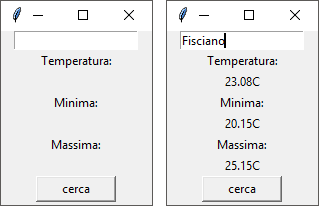
\includegraphics[width=7cm]{img/screen/screen_1.png}
    \end{center}
    \caption{Screenshot dell'appplicazione}
    \label{fig:dessin}
  \end{figure}